\documentclass[landscape]{article}
\usepackage[a4paper, margin=1cm]{geometry}
\usepackage{tikz}
\usetikzlibrary{shapes,arrows,positioning,fit,backgrounds,decorations.pathreplacing,calc,shadows}

\begin{document}

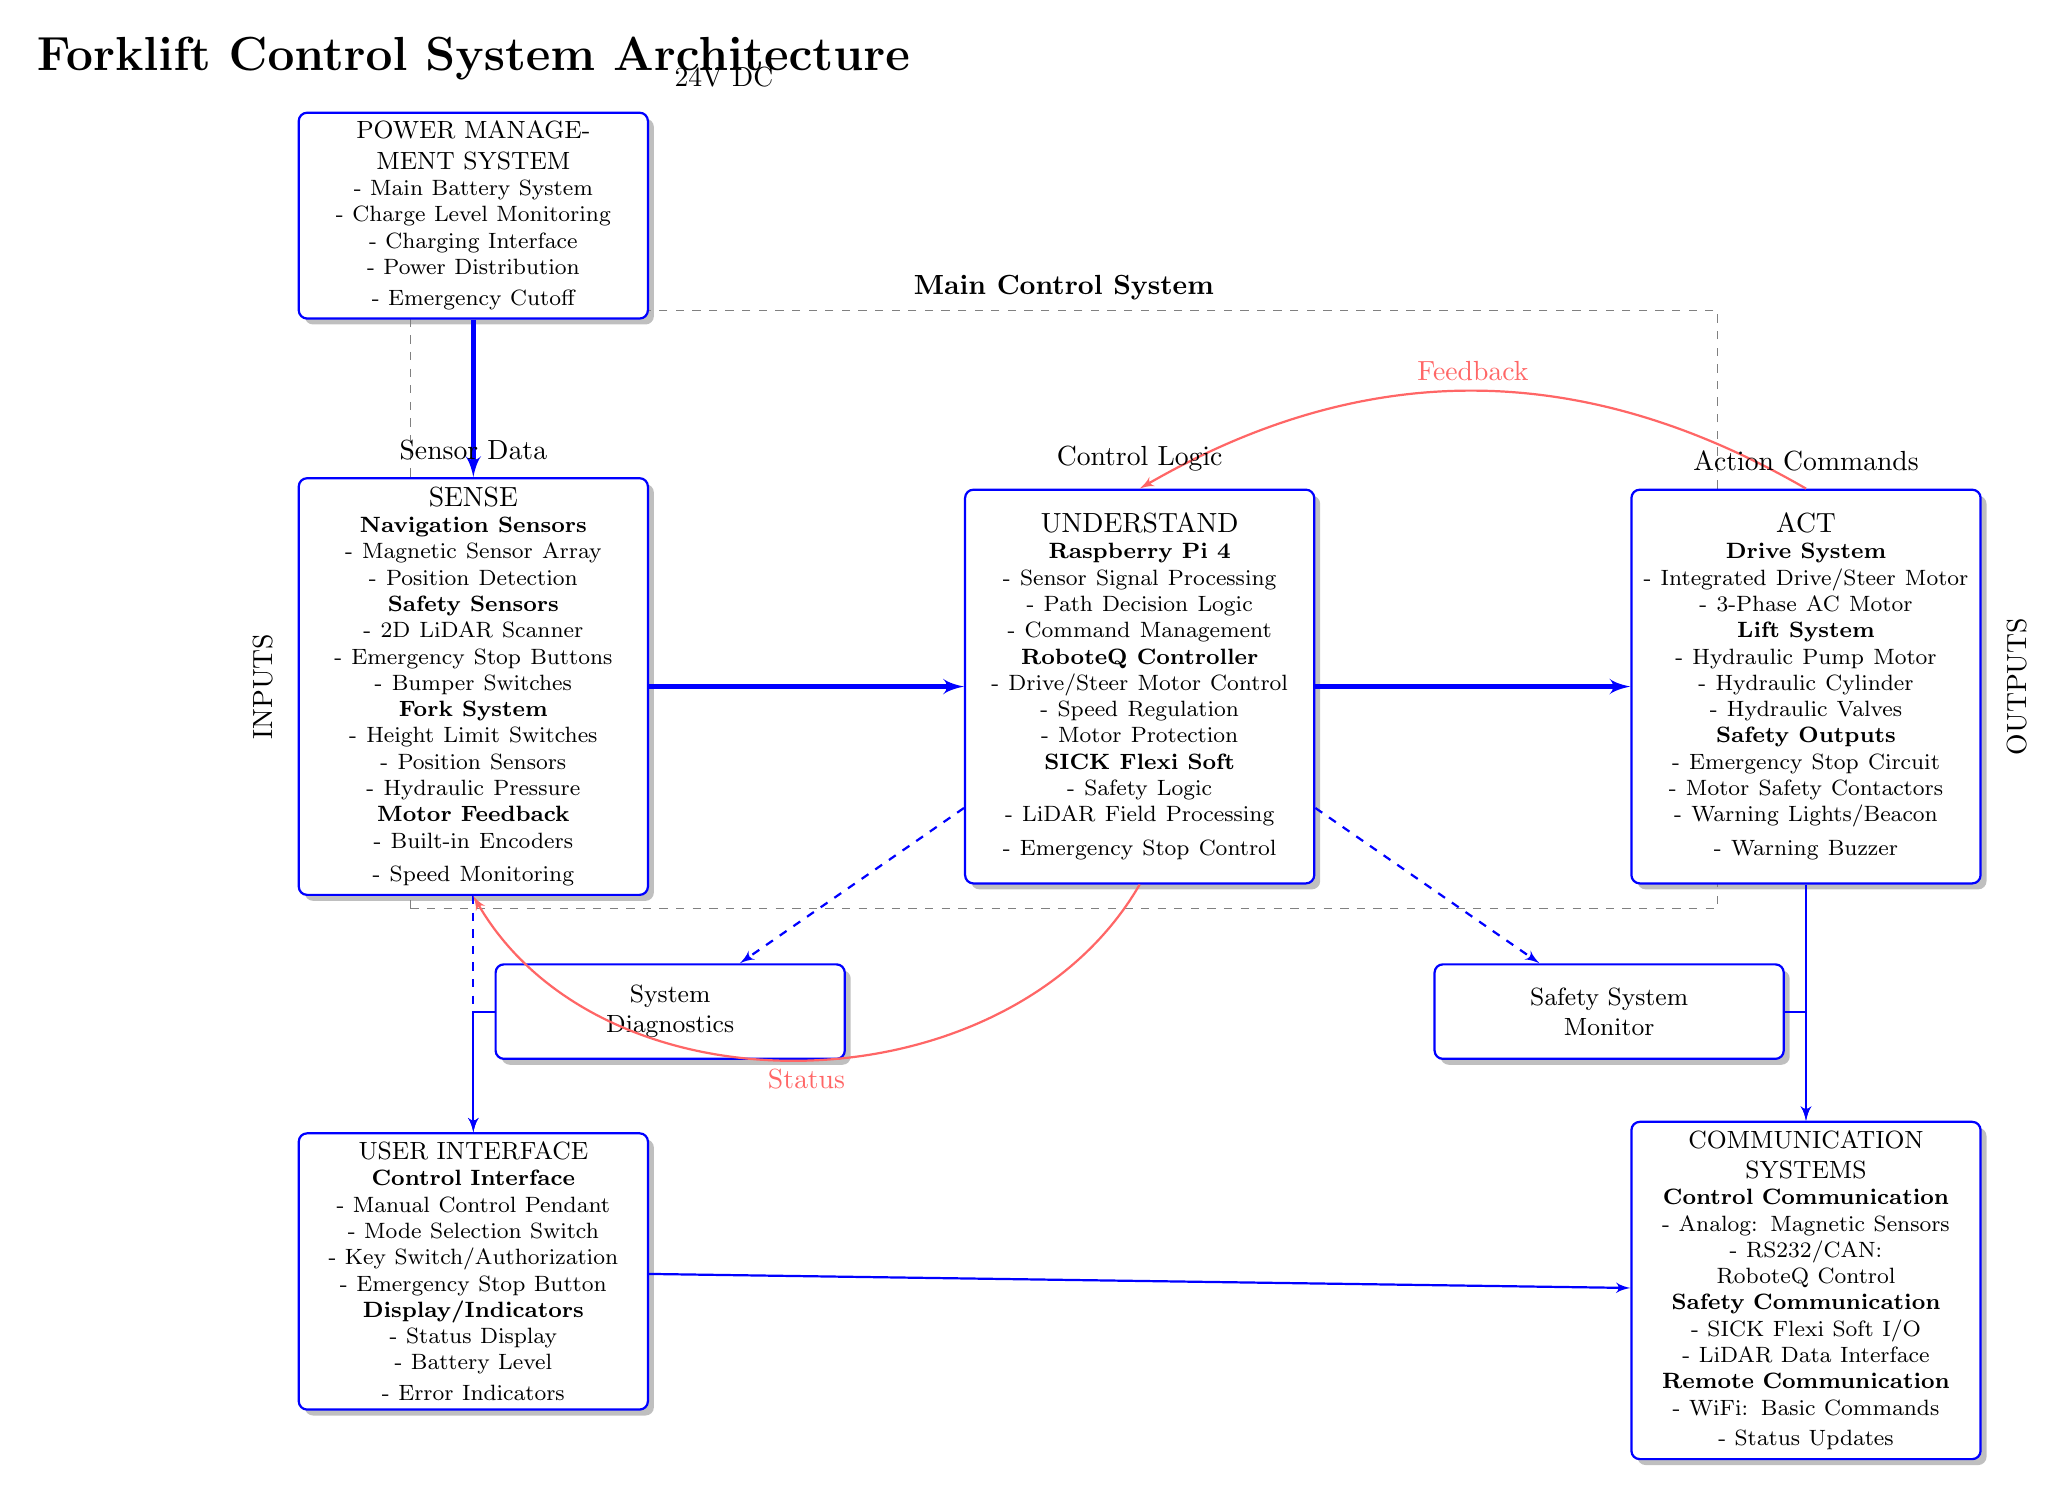
\begin{tikzpicture}[
    auto,
    block/.style={
        rectangle,
        draw=blue,
        thick,
        text width=4.2cm,
        minimum height=1.2cm,
        align=center,
        rounded corners=3pt,
        fill=white,
        drop shadow,
        font=\small
    },
    mainblock/.style={
        rectangle,
        draw=blue,
        thick,
        text width=4.2cm,
        minimum height=5cm,
        align=center,
        rounded corners=3pt,
        fill=white,
        drop shadow
    },
    line/.style={draw, thick, -latex', blue},
    dashed line/.style={draw, thick, dashed, -latex', blue},
    dataflow/.style={draw, thick, -latex', red!60},
    box/.style={
        rectangle,
        draw=gray,
        dashed,
        inner sep=0.8cm
    }
]

% Title
\node [font=\LARGE\bfseries] at (0,4) {Forklift Control System Architecture};

% Power Management System
\node [block] (power) at (0,2) {POWER MANAGEMENT SYSTEM\\
    \footnotesize
    - Main Battery System\\
    - Charge Level Monitoring\\
    - Charging Interface\\
    - Power Distribution\\
    - Emergency Cutoff};

% Main Control System Box
\begin{scope}[on background layer]
    \node[box, fit={($(power)+(0,-2)$) ($(power)+(15,-8)$)}] (controlbox) {};
    \node[above] at (controlbox.north) {\textbf{Main Control System}};
\end{scope}

% Main components
\node [mainblock, below=2cm of power] (sense) {SENSE\\
    \footnotesize
    \textbf{Navigation Sensors}\\
    - Magnetic Sensor Array\\
    - Position Detection\\
    \textbf{Safety Sensors}\\
    - 2D LiDAR Scanner\\
    - Emergency Stop Buttons\\
    - Bumper Switches\\
    \textbf{Fork System}\\
    - Height Limit Switches\\
    - Position Sensors\\
    - Hydraulic Pressure\\
    \textbf{Motor Feedback}\\
    - Built-in Encoders\\
    - Speed Monitoring};

\node [mainblock, right=4cm of sense] (understand) {UNDERSTAND\\
    \footnotesize
    \textbf{Raspberry Pi 4}\\
    - Sensor Signal Processing\\
    - Path Decision Logic\\
    - Command Management\\
    \textbf{RoboteQ Controller}\\
    - Drive/Steer Motor Control\\
    - Speed Regulation\\
    - Motor Protection\\
    \textbf{SICK Flexi Soft}\\
    - Safety Logic\\
    - LiDAR Field Processing\\
    - Emergency Stop Control};

\node [mainblock, right=4cm of understand] (act) {ACT\\
    \footnotesize
    \textbf{Drive System}\\
    - Integrated Drive/Steer Motor\\
    - 3-Phase AC Motor\\
    \textbf{Lift System}\\
    - Hydraulic Pump Motor\\
    - Hydraulic Cylinder\\
    - Hydraulic Valves\\
    \textbf{Safety Outputs}\\
    - Emergency Stop Circuit\\
    - Motor Safety Contactors\\
    - Warning Lights/Beacon\\
    - Warning Buzzer};

% Interface and Communication
\node [block, below=3cm of sense] (ui) {USER INTERFACE\\
    \footnotesize
    \textbf{Control Interface}\\
    - Manual Control Pendant\\
    - Mode Selection Switch\\
    - Key Switch/Authorization\\
    - Emergency Stop Button\\
    \textbf{Display/Indicators}\\
    - Status Display\\
    - Battery Level\\
    - Error Indicators};

\node [block, below=3cm of act] (comm) {COMMUNICATION SYSTEMS\\
    \footnotesize
    \textbf{Control Communication}\\
    - Analog: Magnetic Sensors\\
    - RS232/CAN: RoboteQ Control\\
    \textbf{Safety Communication}\\
    - SICK Flexi Soft I/O\\
    - LiDAR Data Interface\\
    \textbf{Remote Communication}\\
    - WiFi: Basic Commands\\
    - Status Updates};

% Additional control blocks
\node [block, below right=1cm and 1.5cm of understand] (safety) {Safety System\\Monitor};
\node [block, below left=1cm and 1.5cm of understand] (monitor) {System\\Diagnostics};

% Main connections
\draw [line, ultra thick] (power) -- (sense);
\draw [line, ultra thick] (sense) -- (understand);
\draw [line, ultra thick] (understand) -- (act);
\draw [dashed line] (sense) -- (ui);
\draw [line] (ui) -- (comm);
\draw [line] (act) -- (comm);
\draw [dashed line] (understand) -- (safety);
\draw [dashed line] (understand) -- (monitor);
\draw [line] (safety) -| (comm);
\draw [line] (monitor) -| (ui);

% Feedback loops
\draw [dataflow] (act.north) to [out=150, in=30] node[above] {Feedback} (understand.north);
\draw [dataflow] (understand.south) to [out=240, in=300] node[below] {Status} (sense.south);

% System labels
\node [left=0.2cm of sense] {\rotatebox{90}{INPUTS}};
\node [right=0.2cm of act] {\rotatebox{90}{OUTPUTS}};

% Technical annotations
\node [above right=0.2cm and 0.2cm of power] {24V DC};
\node [above=0.1cm of sense] {Sensor Data};
\node [above=0.1cm of understand] {Control Logic};
\node [above=0.1cm of act] {Action Commands};

\end{tikzpicture}

\end{document}